\documentclass[11pt]{article}

% set these commands
\newcommand{\course}{CSCI 347}
\newcommand{\proj}{Homework 03}

\usepackage{macros}
\usepackage{geometry}
\usepackage{tcolorbox}
\usepackage{xcolor}
\usepackage{graphicx}
\usepackage{listings} % for code snippets

% page setup and spacing
\geometry{a4paper, margin=0.75in}
\setlength{\parindent}{1em}
\setlength{\parskip}{1em}
\renewcommand{\baselinestretch}{1.0}

% colors for code snippet
\definecolor{codegreen}{rgb}{0,0.6,0}
\definecolor{codegray}{rgb}{0.5,0.5,0.5}
\definecolor{codepurple}{rgb}{0.58,0,0.82}
\definecolor{backcolour}{rgb}{0.95,0.95,0.92}

% code snippet styling
\lstdefinestyle{mystyle}{
    backgroundcolor=\color{backcolour},   
    commentstyle=\color{codegreen},
    keywordstyle=\color{magenta},
    numberstyle=\tiny\color{codegray},
    stringstyle=\color{codepurple},
    basicstyle=\ttfamily\footnotesize,
    breakatwhitespace=false,         
    breaklines=true,                 
    captionpos=b,                    
    keepspaces=true,                 
    numbers=left,                    
    numbersep=5pt,                  
    showspaces=false,                
    showstringspaces=false,
    showtabs=false,                  
    tabsize=2
}
\lstset{style=mystyle}


\begin{document}

{ ~\\
    River Kelly \\
    \course \\ 
    \proj \\ 
}

Show your work. Include any code snippets you used to generate an answer, using
comments in the code to clearly indicate which problem corresponds to which code

Consider the following graph:

\begin{center}
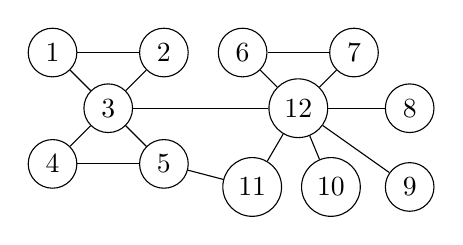
\begin{tikzpicture}[main/.style = {draw, circle}]

\node[main] (3) {3};
\node[main] (1) [above left of=3] {1};
\node[main] (2) [above right of=3] {2};
\node[main] (4) [below left of=3] {4};
\node[main] (5) [below right of=3] {5};


\node[main] (6) [right of=2] {6};
\node[main] (12) [below right of=6] {12};
\node[main] (7) [above right of=12] {7};
\node[main] (8) [below right of=7] {8};
\node[main] (9) [below of=8] {9};
\node[main] (10) [left of=9] {10};
\node[main] (11) [left of=10] {11};

\draw[-] (1) -- (2);
\draw[-] (1) -- (3);
\draw[-] (2) -- (3);

\draw[-] (3) -- (4);
\draw[-] (3) -- (5);
\draw[-] (3) -- (12);

\draw[-] (4) -- (5);
\draw[-] (5) -- (11);

\draw[-] (6) -- (7);
\draw[-] (6) -- (12);
\draw[-] (7) -- (12);
\draw[-] (8) -- (12);
\draw[-] (9) -- (12);
\draw[-] (10) -- (12);
\draw[-] (11) -- (12);

\end{tikzpicture}
\end{center}

\begin{enumerate}

    % Problem 1
    \newpage
    \item (3 points) Without using networkx or other graph analysis packages
    (though you may use them to check your answer), find the closeness
    centrality of vertices 3 and 12.
    \begin{tcolorbox}[width=\linewidth,colback=yellow!5,colframe=yellow!75!black!75,title=Notes]
        Closeness Centrality of $x_i$:
        $$cc(x_{i}) = \frac{1}{\sum_{j=1}^{n} d( x_i , x_j )}$$
        Where $d( x_i , x_j )$ is the shortest path between $x_i$ and $x_j$.
    \end{tcolorbox}
    The closeness centrality of vertices 3:
    \begin{align*}
        cc(x_{3}) &= \frac{1}{\sum_{j=1}^{n} d( x_3 , x_j )} \\
        &= \frac{1}{1 + 1 + 0 + 1 + 1 + 2 + 2 + 2 + 2 + 2 + 2 + 1} \\
        &= \frac{1}{17} \\
        &= 0.05882....
    \end{align*}
    The closeness centrality of vertices 12:
    \begin{align*}
        cc(x_{12}) &= \frac{1}{\sum_{j=1}^{n} d( x_{12} , x_j )} \\
        &= \frac{1}{2+2+1+2+2+1+1+1+1+1+1+0} \\
        &= \frac{1}{15} \\
        &= 0.06666....
    \end{align*}
    \begin{tcolorbox}[width=\linewidth,title=Problem 1 Answer - Closeness Centrality]
        \textit{Note: This solution was done by hand.}\vspace{5pt} \\
        The closeness centrality of vertex 3: $\frac{1}{17}$ or $0.059$ \\
        The closeness centrality of vertex 12: $\frac{1}{15}$ or $0.067$
    \end{tcolorbox}
    
    % Problem 2
    \newpage
    \item (3 points) Without using networkx or other graph analysis packages
    (though you may use them to check your answer), find the eccentricity of
    vertices 3, 12, and 11.
    \begin{tcolorbox}[width=\linewidth,colback=yellow!5,colframe=yellow!75!black!75,title=Notes]
        % Eccentricity: the less eccentric a node is the more central it is. \\
        Eccentricity of $x_i$ is: $$e(x_i) = \max_{i} \lbrace d( x_{i} , x_{j} ) \rbrace$$
    \end{tcolorbox}
    \begin{align*}
        e(x_3) &= 2 \\
        e(x_{12}) &= 2 \\
        e(x_{11}) &= 3
    \end{align*}
    \begin{tcolorbox}[width=\linewidth,title=Problem 2 Answer - Eccentricity]
        \textit{Note: This solution was done by hand.}\vspace{5pt} \\
        The eccentricity of vertex 3: $2$ \\
        The eccentricity of vertex 12: $2$ \\
        The eccentricity of vertex 11: $3$
    \end{tcolorbox}

    % Problem 3
    \newpage
    \item (3 points) Without using networkx or other graph analysis packages
    (though you may use them to check your answer), find the clustering
    coefficient of vertex 3.
    \begin{tcolorbox}[width=\linewidth,colback=yellow!5,colframe=yellow!75!black!75,title=Notes]
        Let $G_i = (V_i, E_i)$ be the subgraph included by the neighbors of node $x_i$. \\
        Let $n_i = \mid V_i \mid$ and $m_i = \mid VE_i \mid$, \\
        Clustering Coefficient of $x_i$:
        $$\frac{ m_{i} }{ ( \substack{ n_{i} \\ 2} ) } = \frac{ \text{\# of edges amoung neighbors of } x_{i} }{ \text{\# of possible edges amoung neighbors of } x_{i} }$$
    \end{tcolorbox}
    \begin{align*}
        \frac{ m_{3} }{ ( \substack{ n_{3} \\ 2} ) } &= \frac{2}{10} \\
        &= \frac{1}{5} \\
        &= 0.2
    \end{align*}
    \begin{tcolorbox}[width=\linewidth,title=Problem 3 Answer - Clustering Coefficient of $x_3$]
        \textit{Note: This solution was done by hand.}\vspace{5pt} \\
        The clustering coefficient of vertex 3 is $\frac{1}{5}$ or $0.2$
    \end{tcolorbox}

    % Problem 4
    \newpage
    \item (3 points) Without using networkx or other graph analysis packages
    (though you may use them to check your answer), find the clustering
    coefficient of the graph.
    $$
        \begin{matrix}
            x_i     &  \frac{ m_{i} }{ ( \substack{ n_{i} \\ 2} ) } \\
            x_1     &  1 \\
            x_2     &  1 \\
            x_3     &  \frac{1}{5} \\
            x_4     &  1 \\
            x_5     &  \frac{1}{3} \\
            x_6     &  1 \\
            x_7     &  1 \\
            x_8     &  0 \\
            x_9     &  0 \\
            x_{10}  &  0 \\
            x_{11}  &  0 \\
            x_{12}  &  \frac{1}{21} \\
        \end{matrix}
    $$
    Clustering Coefficient of the graph:
    \begin{align*}
        C(G) &= \frac{1}{n} \sum_{i=1}^{n} \text{clust coeff } x_i \\
        &= \frac{1}{12} ( 1 + 1 + \frac{1}{5} + 1 + \frac{1}{3} + 1 + 1 + 0 + 0 + 0 + 0 + \frac{1}{21} ) \\
        &= \frac{1}{12} \times \frac{586}{105}  \\
        &= \frac{293}{630} \\
        &= 0.46507\ldots
    \end{align*}
    \begin{tcolorbox}[width=\linewidth,title=Problem 4 Answer - Clustering Coefficient of graph $G$]
        The clustering coefficient of graph $G$ 3 is $\frac{293}{630}$ or $0.46508$
    \end{tcolorbox}


    % Problem 5
    \newpage
    \item (3 points) Find the betweenness centrality of vertices 3 and 12. You
    may use networkx or other graph analysis packages, but include the code used
    to generate your answer in your submission.
\begin{lstlisting}[language=Python]
# libraries
import networkx as nx
import matplotlib.pyplot as plt

# Init Graph
G = nx.Graph()

# Add edges to graph
G.add_edge(1, 2)
G.add_edge(1, 3)
G.add_edge(2, 3)
G.add_edge(3, 4)
G.add_edge(3, 5)
G.add_edge(3, 12)
G.add_edge(4, 5)
G.add_edge(5, 11)
G.add_edge(6, 7)
G.add_edge(6, 12)
G.add_edge(7, 12)
G.add_edge(8, 12)
G.add_edge(9, 12)
G.add_edge(10, 12)
G.add_edge(11, 12)
\end{lstlisting}
Betweenness Centrality:
\begin{lstlisting}[language=Python]
# using definition in the slides
nx.betweenness_centrality(G, normalized=False)
\end{lstlisting}
Output:
\begin{lstlisting}
{
    1: 0.0,
    2: 0.0,
    3: 27.0,
    4: 0.0,
    5: 2.5,
    12: 40.5,
    11: 3.0,
    6: 0.0,
    7: 0.0,
    8: 0.0,
    9: 0.0,
    10: 0.0
}
\end{lstlisting}

    \begin{tcolorbox}[width=\linewidth,title=Problem 5 Answer - Betweenness]
        The betweenness centrality of vertices 3 and 12 is $27$ and $40.5$, respectively.
    \end{tcolorbox}

    % Problem 6
    \newpage
    \item (3 points) Using networkx, find the prestige centrality of vertices 3
    and 12. Include the code used to generate the answer. (Note that networkx
    calls the prestige centrality ``eigenvector centrality'')
\begin{lstlisting}[language=Python]
# prestige centrality
nx.eigenvector_centrality(G)
\end{lstlisting}
Output:
\begin{lstlisting}
{
    1: 0.21086454283237194,
    2: 0.21086454283237194,
    3: 0.46528704789070097,
    4: 0.23879994540475255,
    5: 0.3004407253859518,
    12: 0.5310014523926223,
    11: 0.25929496322149226,
    6: 0.24064930403878465,
    7: 0.24064930403878465,
    8: 0.1655995303513709,
    9: 0.1655995303513709,
    10: 0.1655995303513709
}
\end{lstlisting}

    \begin{tcolorbox}[width=\linewidth,title=Problem 6 Answer - Eigenvector Centrality]
        The prestige centrality of vertices 3 and 12 is $0.4653$ and $0.5310$, respectively.
    \end{tcolorbox}

    % Problem 7
    \newpage
    \item (3 points) Use Python to create a plot for the degree distribution of
    this graph.  Include the code used to generate the plot as well as the plot
    in your submission.
\begin{lstlisting}[language=Python]
deg_view = nx.degree(G)
deg_vals = dict(deg_view).values()

plt.hist(deg_vals)
plt.xlabel('degree')
plt.ylabel('number of nodes with degree')
\end{lstlisting}

    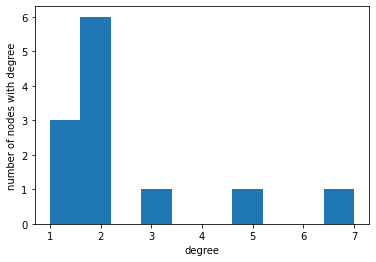
\includegraphics[width=\linewidth]{q7-node-degree.png}

\end{enumerate}

{\bf Acknowledgements:} Homework problems adapted from assignments of
Veronika Strnadova-Neeley.

\end{document}
